
\section{Giao diện Website dự án}
Để chứng minh kết quả phát triển giao diện hệ thống giám sát và điều khiển nhà thông minh \texttt{YOLOHome}, dưới đây là danh sách các ảnh chụp màn hình ghi nhận giao diện vận hành thực tế của hệ thống. Các tệp ảnh chụp giao diện được lưu trữ tại thư mục \texttt{figures/} dưới các tên tương ứng và được liên kết bằng các mã hình vẽ để dễ dàng kiểm tra.

Hệ thống cung cấp màn hình Đăng nhập (\texttt{/}) và màn hình Đăng ký (\texttt{/signup}) có thiết kế giao diện theo phong cách Sleek Dark-mode tối giản và trực quan, hỗ trợ người dùng bảo mật tài khoản cá nhân. Sau khi đăng nhập thành công, người dùng được điều hướng đến trang Dashboard hiển thị thông số cảm biến môi trường thời gian thực.

\begin{figure}[H]
    \centering
    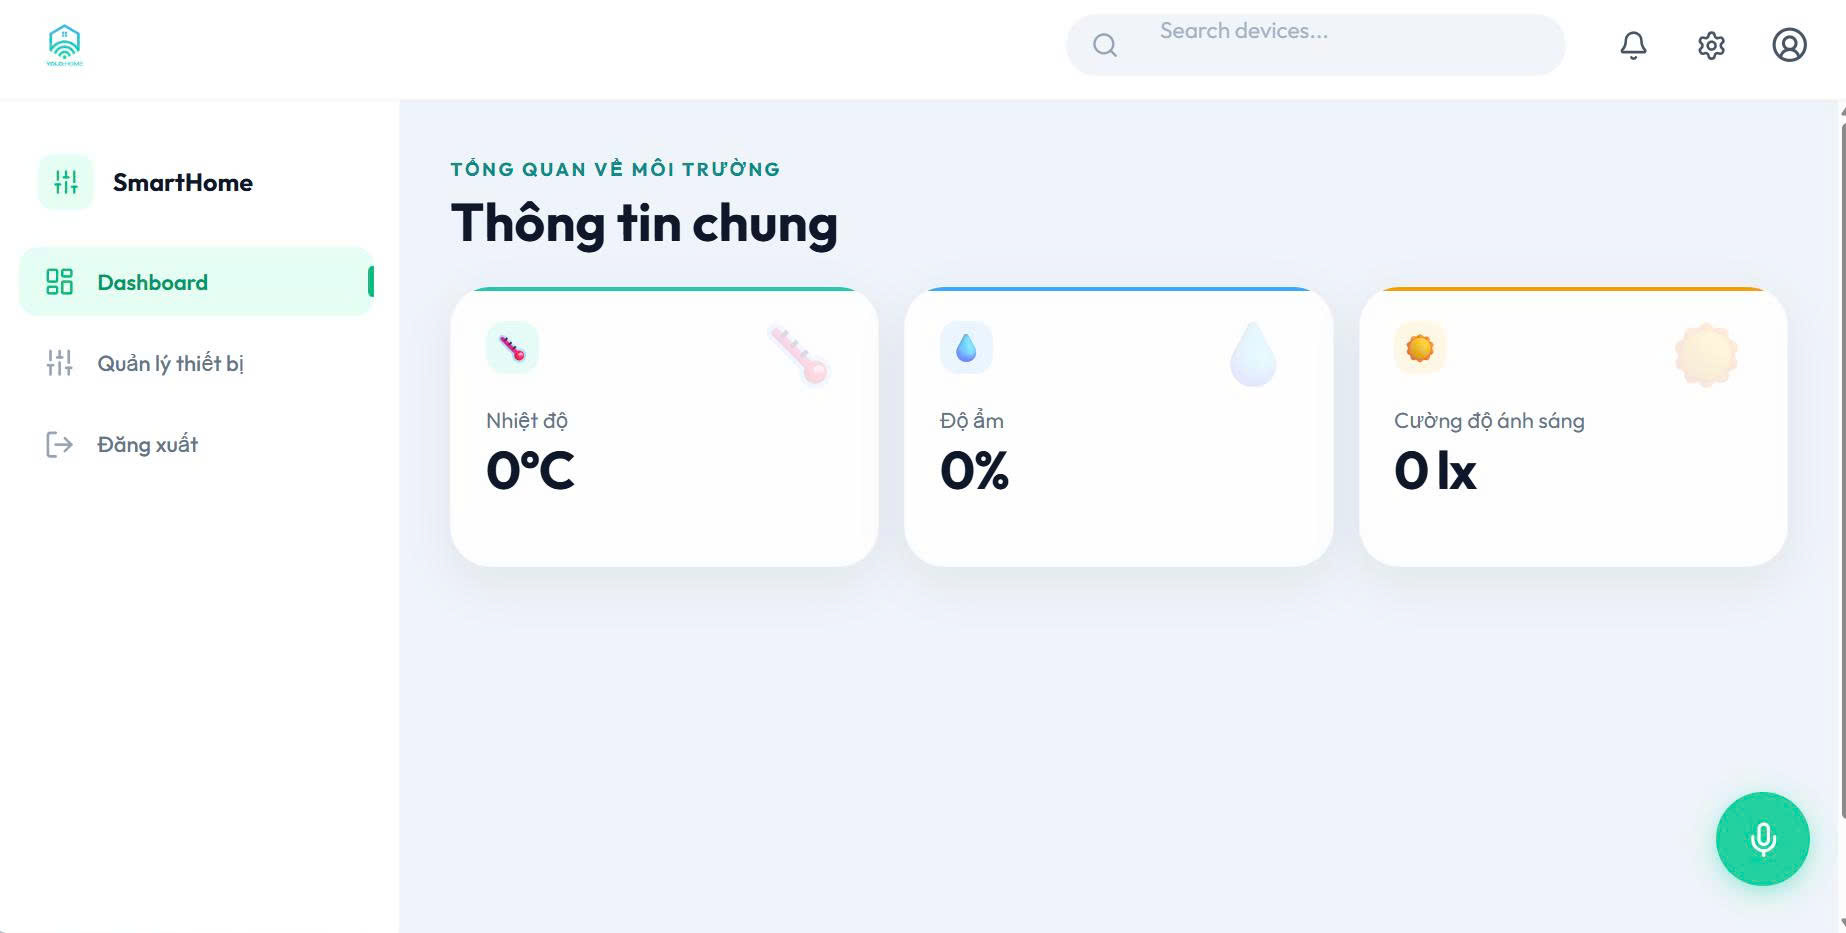
\includegraphics[width=0.95\textwidth]{figures/ui-dashboard.jpg}
    \caption{Ảnh chụp giao diện Dashboard hiển thị thông số cảm biến môi trường}
    \label{fig:ui-dashboard}
\end{figure}

Giao diện Dashboard tại \autoref{fig:ui-dashboard} cập nhật dữ liệu liên tục sau mỗi 5 giây. Khi phát hiện các chỉ số cảm biến vượt qua ngưỡng cấu hình an toàn, hệ thống tự động sinh cảnh báo và hiển thị hộp thông tin màu đỏ nổi bật trực quan như trình bày tại \autoref{fig:ui-alert}.

\begin{figure}[H]
    \centering
    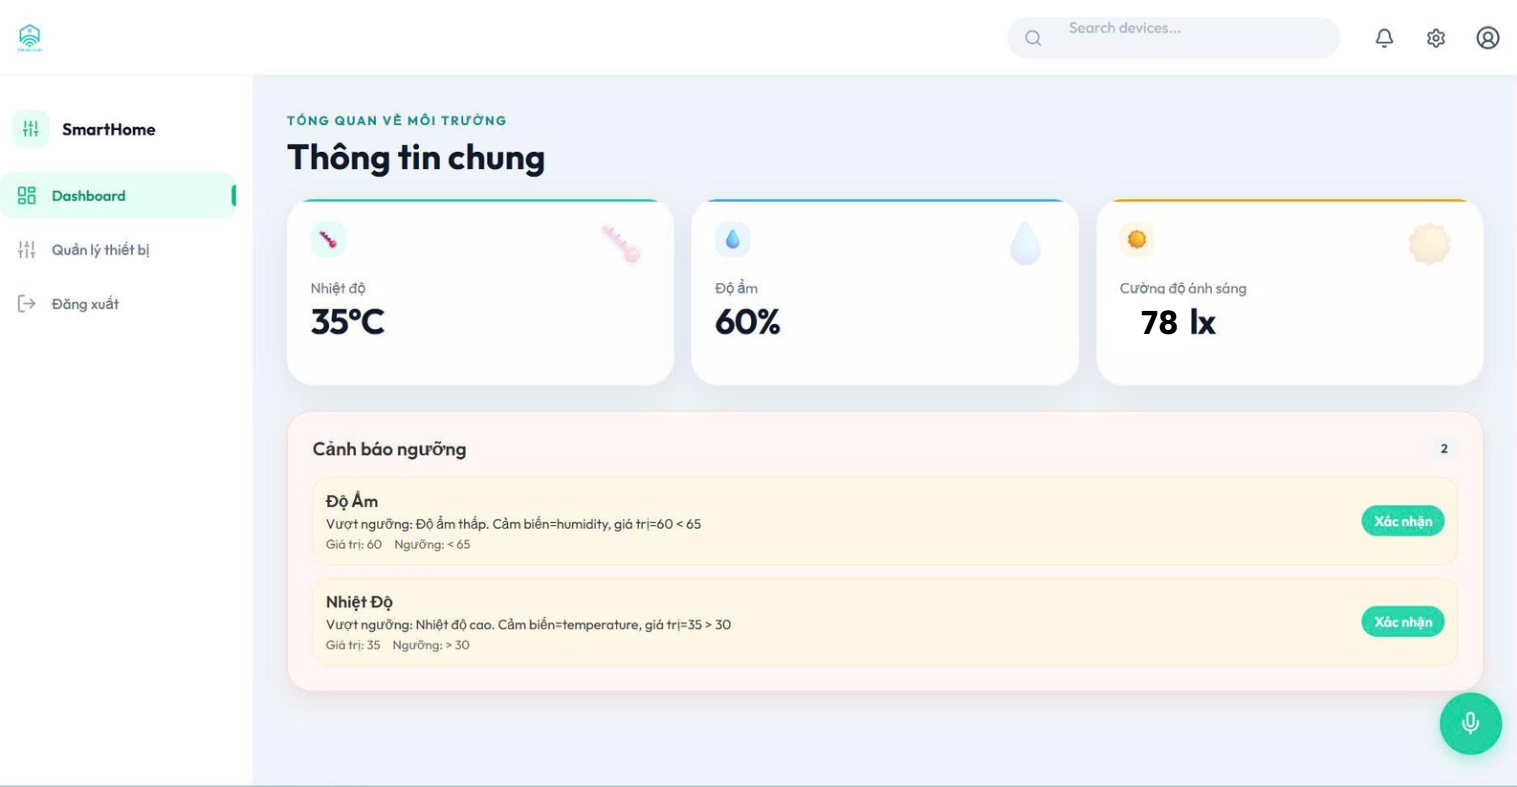
\includegraphics[width=0.95\textwidth]{figures/ui-alert.png}
    \caption{Ảnh chụp giao diện hiển thị hộp cảnh báo vi phạm ngưỡng trên Dashboard}
    \label{fig:ui-alert}
\end{figure}

Người dùng có thể chuyển hướng sang trang Quản lý thiết bị (\texttt{/devices}) để kiểm soát và theo dõi trạng thái hiện thời của các thiết bị chấp hành trong nhà bao gồm đèn LED, quạt thông gió và động cơ rèm cửa rực rỡ như mô tả trong \autoref{fig:ui-devices}.

\begin{figure}[H]
    \centering
    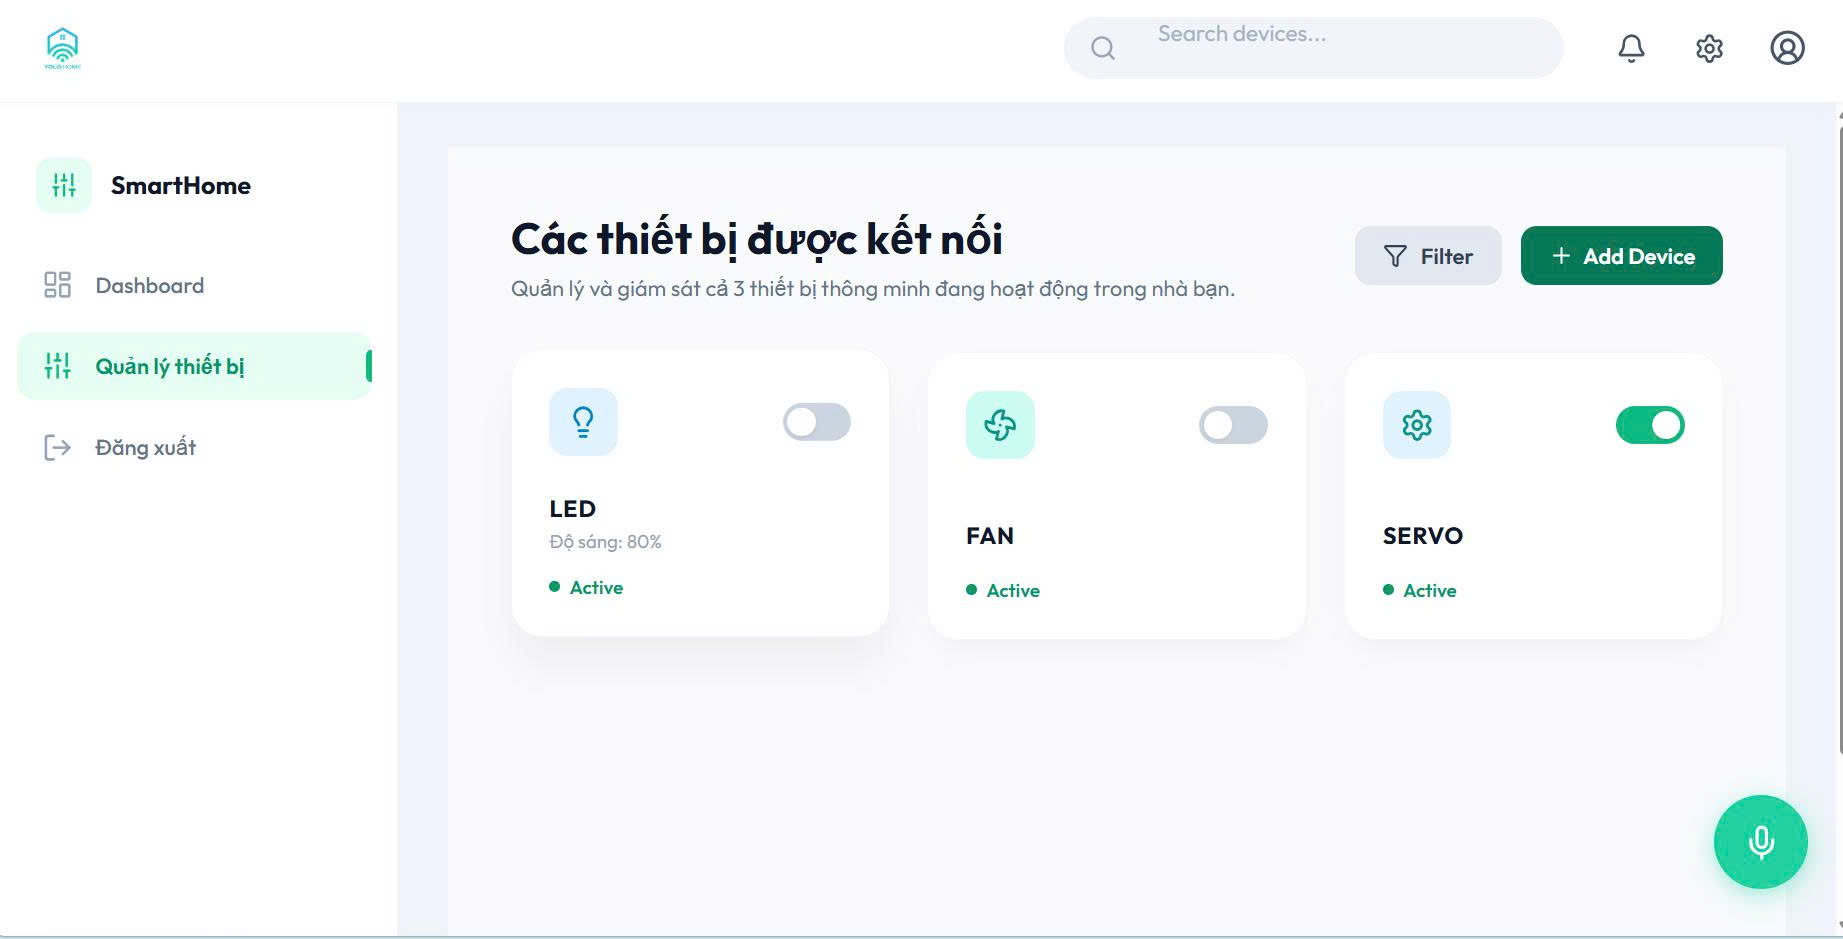
\includegraphics[width=0.95\textwidth]{figures/ui-devices.jpg}
    \caption{Ảnh chụp giao diện trang Quản lý thiết bị và trạng thái bật/tắt thủ công}
    \label{fig:ui-devices}
\end{figure}

Cuối cùng, tính năng điều khiển bằng giọng nói tiếng Việt trôi nổi tích hợp ở góc phải chân màn hình Web hiển thị vòng tròn đỏ phát xung lan tỏa khi ghi âm và Toast báo kết quả được ghi nhận tại \autoref{fig:ui-voice}.

\begin{figure}[H]
    \centering
    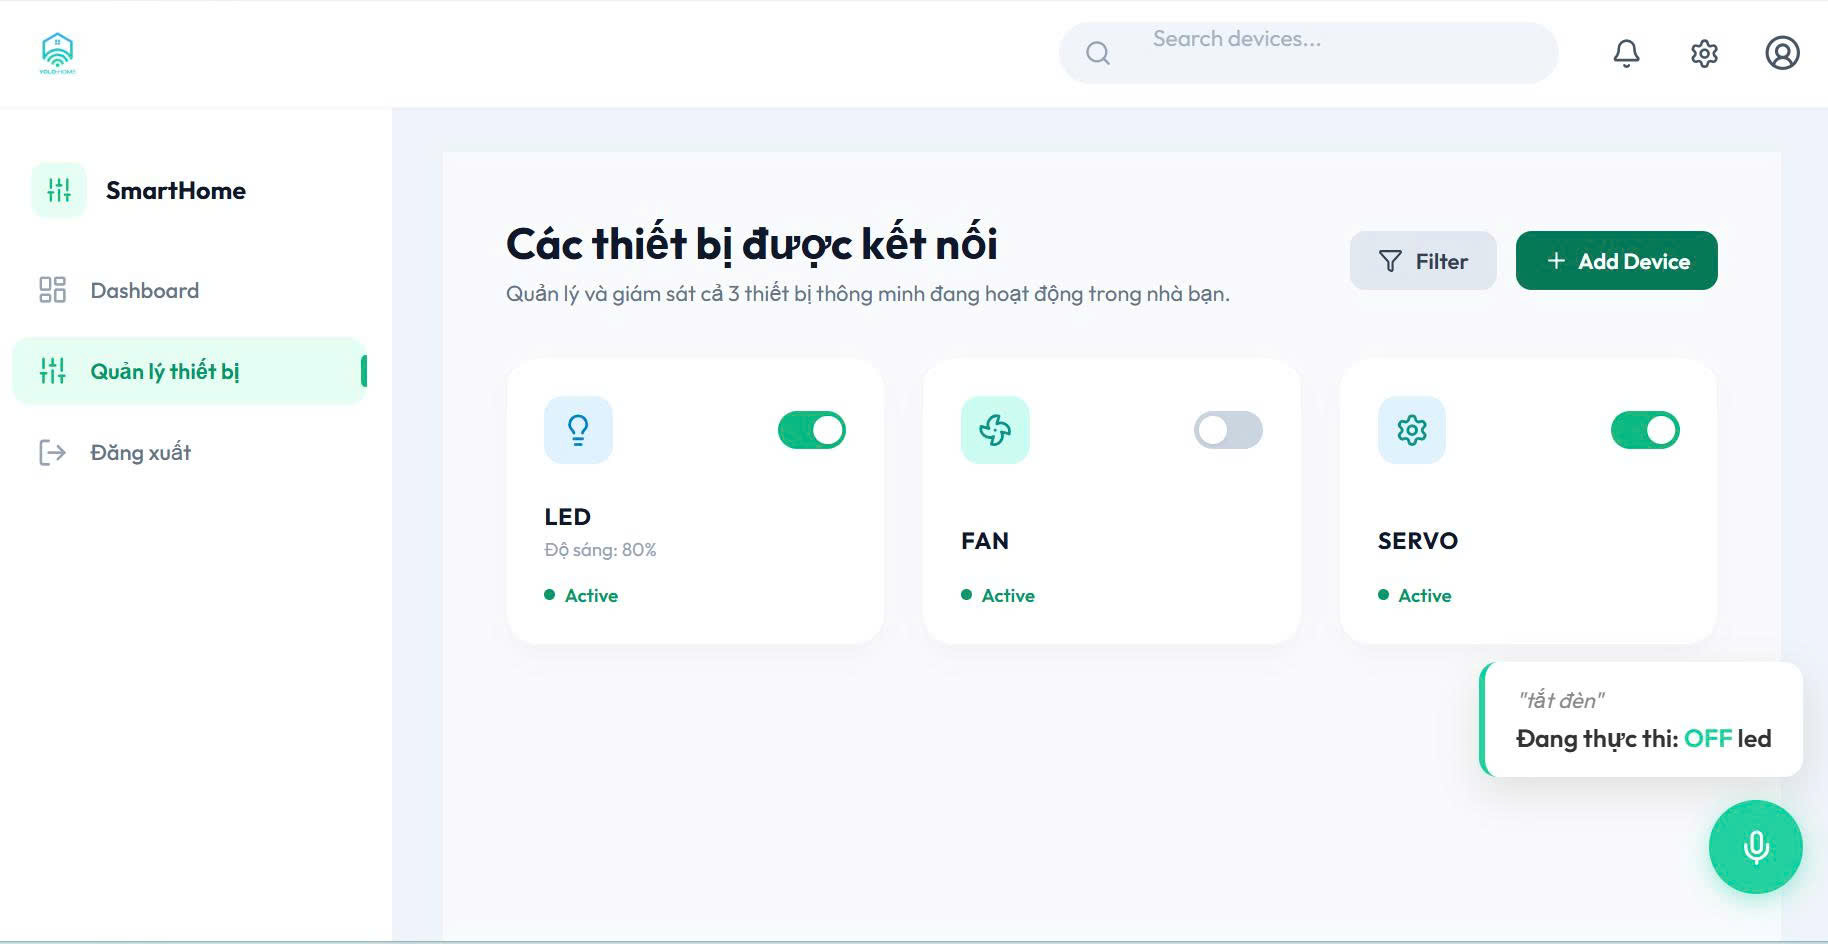
\includegraphics[width=0.95\textwidth]{figures/ui-voice.jpg}
    \caption{Ảnh chụp giao diện nút ghi âm giọng nói tiếng Việt và Toast phản hồi kết quả}
    \label{fig:ui-voice}
\end{figure}

% \section{Video demo}
% Kịch bản video thuyết minh thực tế vận hành hệ thống \texttt{YOLOHome} có thời lượng khoảng 2--3 phút để minh họa trực quan quy trình hoạt động tích hợp từ phần cứng lên phần mềm được chia làm 4 phân đoạn chính:

% \begin{itemize}
%     \item \textbf{Phân đoạn 1 --- Giới thiệu giao diện giám sát cảm biến}:
%         \begin{itemize}
%             \item \emph{Màn hình hiển thị}: Mở trình duyệt Web tại trang Dashboard \texttt{/dashboard} song song với cửa sổ terminal đang chạy logs của Backend Express.
%             \item \emph{Thuyết minh}: "Xin chào thầy cô và các bạn, đây là giao diện Dashboard giám sát các thông số môi trường của hệ thống YOLOHome. Các thông số nhiệt độ, độ ẩm và cường độ ánh sáng đang được thu thập trực tiếp từ cảm biến phần cứng thông qua Gateway và cập nhật lên màn hình mỗi 5 giây."
%             \item \emph{Chứng thực mã nguồn}: Hàm gọi polling dữ liệu cập nhật sau mỗi 5 giây (\texttt{Dashboard.js:75}).
%         \end{itemize}
%     \item \textbf{Phân đoạn 2 --- Điều khiển thiết bị thủ công từ xa}:
%         \begin{itemize}
%             \item \emph{Màn hình hiển thị}: Chuyển sang trang Quản lý thiết bị \texttt{/devices}, mở song song cửa sổ logs của Gateway Python và camera quay trực tiếp Kit phần cứng Yolo:Bit.
%             \item \emph{Thao tác}: Nhấp chuột gạt công tắc bật quạt Fan trên giao diện Web.
%             \item \emph{Thuyết minh}: "Bây giờ tôi sẽ thực hiện bật quạt thông gió từ xa. Khi tôi nhấn nút trên giao diện, trình duyệt gửi yêu cầu HTTP POST tới Backend, Backend sẽ xuất bản tin MQTT điều khiển đến Gateway. Như các bạn thấy trên log của Gateway, lệnh Serial \texttt{!F:1\#} đã được truyền xuống Kit phần cứng thành công và quạt vật lý đã quay."
%             \item \emph{Chứng thực mã nguồn}: Hàm đẩy lệnh qua MQTT (\texttt{deviceController.js:66}) và Gateway truyền Serial UART (\texttt{controller.py:286}).
%         \end{itemize}
%     \item \textbf{Phân đoạn 3 --- Tự động hóa và cảnh báo vi phạm ngưỡng}:
%         \begin{itemize}
%             \item \emph{Màn hình hiển thị}: Quay lại màn hình giao diện Dashboard chính \texttt{/dashboard}.
%             \item \emph{Thao tác}: Gửi tin nhắn giả lập giá trị nhiệt độ cao vượt ngưỡng thông qua công cụ MQTT với giá trị 32$^\circ$C.
%             \item \emph{Thuyết minh}: "Khi cảm biến nhiệt độ báo về giá trị 32 độ C, vượt ngưỡng an toàn cấu hình là 30 độ C. Ngay lập tức, Gateway tự động kích hoạt quạt thông gió vật lý bằng lệnh \texttt{!F:1\#}. Phía Backend cũng phát hiện vi phạm ngưỡng, tạo cảnh báo trong Database và hiển thị thông tin chi tiết kèm nút 'Xác nhận' trên Dashboard của người dùng. Sau khi xử lý sự cố, tôi nhấn nút 'Xác nhận', cảnh báo sẽ biến mất."
%             \item \emph{Chứng thực mã nguồn}: Hàm xử lý tự động hóa Gateway (\texttt{threshold\_service.py:170--191}) và hàm sinh cảnh báo MongoDB (\texttt{alertService.js:230}).
%         \end{itemize}
%     \item \textbf{Phân đoạn 4 --- Điều khiển bằng giọng nói tiếng Việt (Push-to-Talk)}:
%         \begin{itemize}
%             \item \emph{Màn hình hiển thị}: Trình duyệt Web hiển thị nút Microphone trôi nổi ở chân trang Layout.
%             \item \emph{Thao tác}: Nhấp và giữ nút Mic, phát âm câu lệnh "bật đèn" và nhả chuột.
%             \item \emph{Thuyết minh}: "Cuối cùng là chức năng điều khiển bằng giọng nói. Tôi nhấn giữ nút microphone và nói 'bật đèn'. Hệ thống sẽ ghi âm đoạn nói này, gọi tới dịch vụ STT Vosk để chuyển thành văn bản và dùng mô hình ML nhận diện ý định. Hệ thống thông báo thành công và hiển thị toast phản hồi kết quả trực quan."
%             \item \emph{Chứng thực mã nguồn}: Luồng xử lý giọng nói đồng bộ gọi Vosk, ML và đẩy tin nhắn MQTT (\texttt{voiceService.js:162--220}).
%         \end{itemize}
% \end{itemize}

% Đường dẫn xem video minh họa vận hành thực tế hệ thống YOLOHome: \href{https://github.com/AiemHao/YOLOHome}{Video Demo Giám Sát Và Điều Khiển YOLOHome}.

